\documentclass[11pt,a4paper]{article}
% Shared preamble of the FEBAUTO Racing manuals.
\usepackage[margin=2.2cm,headheight=16pt]{geometry}
\usepackage[T1]{fontenc}
\usepackage{lmodern}
\usepackage{xcolor}
\usepackage{graphicx}
\usepackage{booktabs}
\usepackage{tabularx}
\usepackage{listings}
\usepackage{fancyhdr}
\usepackage{enumitem}
\usepackage{tikz}
\usetikzlibrary{arrows.meta}
\usepackage[hidelinks,colorlinks=true,linkcolor=febblue,urlcolor=febblue]{hyperref}

\definecolor{febblue}{HTML}{1C4687}
\definecolor{febgold}{HTML}{FDB515}
\definecolor{codebg}{HTML}{F3F4F6}

\lstset{
  basicstyle=\ttfamily\small,
  backgroundcolor=\color{codebg},
  frame=single, framerule=0pt, framesep=4pt,
  xleftmargin=4pt, xrightmargin=4pt,
  breaklines=true, columns=fullflexible, keepspaces=true,
  showstringspaces=false,
}
\newcommand{\file}[1]{\texttt{#1}}
\newcommand{\cmd}[1]{\texttt{#1}}
\newcommand{\rulebox}[1]{\par\noindent\colorbox{codebg}{\parbox{\dimexpr\linewidth-2\fboxsep}{#1}}\par\medskip}

\pagestyle{fancy}
\fancyhf{}
\fancyhead[L]{\color{febblue}\textbf{FEBAUTO Racing}}
\fancyhead[R]{\color{febblue}\nouppercase{\leftmark}}
\fancyfoot[C]{\thepage}
\renewcommand{\headrulewidth}{0.8pt}
\renewcommand{\headrule}{\color{febgold}\hrule width\headwidth height\headrulewidth}
\setcounter{tocdepth}{1}

% \febtitle{subtitle}{part lines}
\newcommand{\febtitle}[2]{%
\begin{titlepage}
  \centering
  \vspace*{2cm}
  
\includegraphics[width=5cm]{../../assets/feb_logo_512.png}\\[1.5cm]
  {\color{febblue}\Huge\bfseries FEBAUTO Racing}\\[6pt]
  {\Large #1}\\[2cm]
  \begin{tabular}{rl}#2\end{tabular}\\[3cm]
  Formula Electric at Berkeley\\
  September 2026, platform release v0.1.0\\[6pt]
  \url{https://github.com/FEBAutonomous/feb-racing}\\
  \url{https://febautonomous.github.io/feb-racing/}
\end{titlepage}
\tableofcontents
\newpage}

\usetikzlibrary{positioning,fit,backgrounds,calc,shapes.misc}
\tikzset{
  box/.style={draw=febblue,thick,rounded corners=3pt,fill=white,align=center,inner sep=6pt,font=\small},
  soft/.style={draw=febblue!60,thick,rounded corners=3pt,fill=febblue!6,align=center,inner sep=6pt,font=\small},
  state/.style={draw=febblue,thick,rounded corners=6pt,fill=white,align=center,inner sep=7pt,font=\small\bfseries,minimum width=24mm},
  stop/.style={state,fill=red!8,draw=red!60!black},
  go/.style={state,fill=green!10,draw=green!40!black},
  outer/.style={draw=febblue!40,dashed,rounded corners=6pt,inner sep=10pt},
  lbl/.style={font=\scriptsize\color{febblue},fill=white,inner sep=1pt},
  flow/.style={-{Stealth[length=6pt]},thick,febblue},
  both/.style={{Stealth[length=6pt]}-{Stealth[length=6pt]},thick,febblue},
}
\setlist{nosep,leftmargin=*}

\begin{document}
\febtitle{Member guide, release 2}{%
  \textbf{Part I} & The box: your ROS 2 environment\\[3pt]
  \textbf{Part II} & Drivers: write, score, submit\\[3pt]
  \textbf{Part III} & The car\\}

\noindent{\small\color{gray}Verified end to end, every command as written, on Linux (Ubuntu 22.04) and macOS
(Apple Silicon) on 2026-10-21, and on Windows~11 (PowerShell, Docker Desktop) on 2026-10-24.}

\section{What changed, in one minute}

Release 2 replaces the throwaway devkit container with \textbf{the box}: a Linux machine with ROS~2
Humble inside Docker that keeps what you install, sees your whole FEB folder, and runs the same on
the car's Jetson. Your driver talks the real car's topics, so what laps in the simulator drives the
car unchanged. The launcher is \cmd{feb}; \cmd{feb-sim} is gone.

\begin{tabularx}{\linewidth}{lX}
\toprule
Was & Is \\
\midrule
\cmd{./feb-sim run} & \cmd{./feb up} \\
\cmd{./feb-sim shell} & \cmd{./feb shell}, or \cmd{./feb code} for VS Code inside the box \\
container wiped on every run & the box persists; \cmd{./feb reset} wipes it on purpose \\
only \file{stack/} visible inside & all of \file{\textasciitilde/FEB} visible inside \\
topics \texttt{/autodrive/roboracer\_1/*}, throttle in $[0,1]$ & \texttt{/scan}, \texttt{/odom}, \texttt{/imu}, camera in; \texttt{/drive} (m/s, rad) out \\
one practice track & every practice track of your driver's kind \\
submit posts a result & submit posts the results and your code \\
\bottomrule
\end{tabularx}

\part{The box}

\section{Setup}

\subsection*{1. Install, once}

\begin{tabularx}{\linewidth}{lX}
\toprule
 & Install \\
\midrule
Mac & Docker Desktop (or OrbStack). VS~Code, then its Extensions view, search \emph{Dev Containers}, Install. Foxglove from \url{https://foxglove.dev/download}. \\
Windows & In PowerShell \cmd{wsl -{}-install}, then \cmd{wsl -{}-update}, reboot: that is Docker's engine, you never open Ubuntu. Then Docker Desktop. Python~3 from \url{https://python.org} with \emph{Add python.exe to PATH} ticked. Git for Windows from \url{https://git-scm.com}. VS~Code with the Dev Containers extension (Extensions view, search, Install). Foxglove. \\
Linux & \cmd{sudo apt install docker.io}, \cmd{sudo usermod -aG docker \$USER}, log out and in. VS~Code with Dev Containers. Foxglove. \\
\bottomrule
\end{tabularx}

\medskip
Sign-ins: Docker Desktop offers one, skip it. Foxglove needs a free account the first time it opens.
VS~Code needs none.

And one GitHub thing: an SSH key on your account. If the clone below stops with \texttt{Permission
denied (publickey)}, this machine has no key on your GitHub account yet. Either \cmd{ssh-keygen -t
ed25519}, Enter three times, then paste the contents of \file{\textasciitilde/.ssh/id\_ed25519.pub}
into GitHub, Settings, SSH and GPG keys, New SSH key, and clone again. Or clone over https,
\cmd{https://github.com/FEBAutonomous/feb-racing.git}, and add the key before your first
\cmd{feb submit}. On Windows, \cmd{ssh-keygen} runs in PowerShell too, and the key is in \file{C:\textbackslash Users\textbackslash you\textbackslash .ssh}.

Where things live: Mac, under \file{/Users}, which \file{\textasciitilde/FEB} already is. Windows:
every command in this guide is typed in \textbf{PowerShell}, the same \cmd{./feb} commands, and
\file{\textasciitilde/FEB} is \file{C:\textbackslash Users\textbackslash you\textbackslash FEB}. The box is Linux
inside Docker; the simulator is the native Windows build on your own GPU. Foxglove is optional
everywhere; the browser desktop covers most of it.

\subsection*{2. Had the old devkit? Delete it}

Release 2 rewrote the repository, so the old clone cannot be updated. Delete it; skip this if
you never had it.

\begin{lstlisting}
rm -rf ~/feb-racing            # or wherever it is;  Windows: rm -r -fo ~/feb-racing
\end{lstlisting}

Wrote code in its \file{stack/} folder? Copy that folder somewhere safe before deleting, and drop
it into the new \file{stack/} after step~3. It runs again once it has a card (section~\ref{sec:package}).

\subsection*{3. Clone and set up}

\begin{lstlisting}
mkdir -p ~/FEB && cd ~/FEB
git clone git@github.com:FEBAutonomous/feb-racing.git && cd feb-racing
./feb setup --name "Your Name"
\end{lstlisting}

Windows, PowerShell, one line at a time (no \cmd{\&\&} there):

\begin{lstlisting}
mkdir ~/FEB; cd ~/FEB
git clone git@github.com:FEBAutonomous/feb-racing.git; cd feb-racing
./feb setup --name "Your Name"
\end{lstlisting}

\texttt{setup} pulls the image (a few GB, once), downloads the simulator app for your OS, and
creates your box. About twenty minutes, nearly all of it download. Your name is how results
appear on the scoreboard; ask the lead to add it to \file{submissions.yaml} with your GitHub
login.

\subsection*{4. First drive}

\begin{lstlisting}
./feb up
\end{lstlisting}

The simulator opens, and Foxglove with it if it is installed. Arrow keys drive. Close the
simulator window, or Ctrl-C in the terminal, to stop. Closing the \emph{terminal} instead leaves the run
going; \cmd{./feb stop} ends it. \cmd{./feb up -{}-driver
feb\_driver} races the starter driver instead. Mac, first time only: if macOS refuses to open the
simulator, right-click \file{FEB Simulator.app} in \file{\textasciitilde/.feb-sim/app/mac} (Finder:
Cmd-Shift-G, paste the path) and choose Open.

That was the one and only clone. Every later release arrives with \cmd{./feb update}.

\section{How it fits together}

\begin{center}
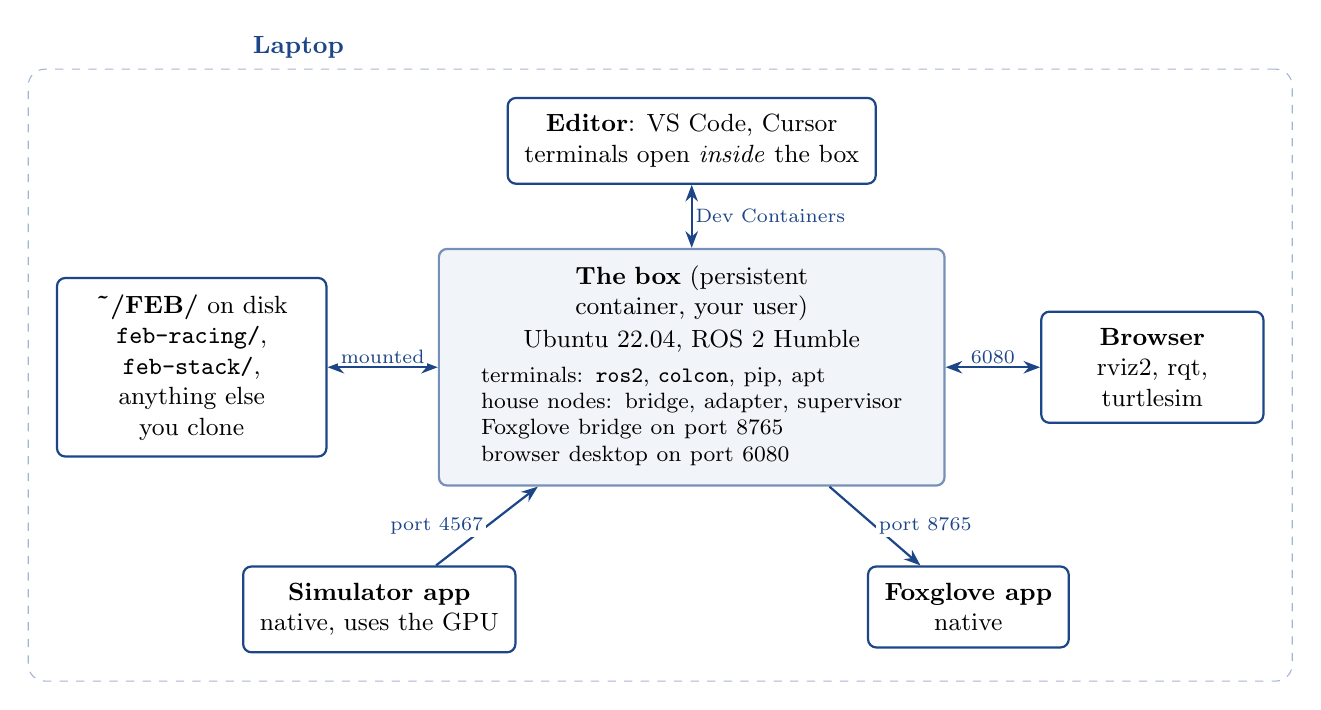
\begin{tikzpicture}[node distance=8mm, font=\small]
  \node[soft, text width=60mm] (box) {
    \textbf{The box} (persistent container, your user)\\[1pt]
    Ubuntu 22.04, ROS 2 Humble\\[3pt]
    {\footnotesize\begin{tabular}{@{}l@{}}
      terminals: \cmd{ros2}, \cmd{colcon}, pip, apt\\
      house nodes: bridge, adapter, supervisor\\
      Foxglove bridge on port 8765\\
      browser desktop on port 6080
    \end{tabular}}};
  \node[box, above=of box] (editor) {\textbf{Editor}: VS Code, Cursor\\terminals open \emph{inside} the box};
  \node[box, left=14mm of box, text width=30mm] (files) {\textbf{\textasciitilde/FEB/} on disk\\\file{feb-racing/}, \file{feb-stack/},\\anything else you clone};
  \node[box, right=12mm of box, text width=24mm] (web) {\textbf{Browser}\\rviz2, rqt,\\turtlesim};
  \node[box, below left=10mm and -10mm of box] (sim) {\textbf{Simulator app}\\native, uses the GPU};
  \node[box, below right=10mm and -10mm of box] (fox) {\textbf{Foxglove app}\\native};
  \draw[both] (files) -- node[lbl,above]{mounted} (box);
  \draw[both] (editor) -- node[lbl,right]{Dev Containers} (box);
  \draw[flow] (sim) -- node[lbl,left]{port 4567} (box);
  \draw[flow] (box) -- node[lbl,right]{port 8765} (fox);
  \draw[both] (box) -- node[lbl,above]{6080} (web);
  \begin{scope}[on background layer]
    \node[outer, fit=(files)(box)(editor)(sim)(fox)(web), label={[febblue,font=\small\bfseries]above left:Laptop}] {};
  \end{scope}
\end{tikzpicture}
\end{center}

The box is one container, made once by \texttt{setup}, started by whichever command needs it,
kept until \cmd{./feb reset}. Your \file{\textasciitilde/FEB} folder is mounted into it at
\file{/home/feb/FEB}: the same files, not a copy, so edit on the laptop with anything or inside
the box, it makes no difference. What you \cmd{apt} or \cmd{pip} install lives in the box and goes
with a reset or a new image; your files never do.

\section{The commands}

\begin{tabularx}{\linewidth}{>{\ttfamily\small}p{6.2cm}X}
\toprule
\normalfont Command & What it does \\
\midrule
./feb shell & a terminal in the box, in the folder you ran it from; open as many as you like \\
./feb shell -{}-gui & the same, plus the box's desktop in a browser tab (rviz2, rqt, turtlesim) \\
./feb code & VS Code attached to the box (\cmd{-{}-cursor} for Cursor) \\
./feb up & house nodes, simulator, Foxglove; drive by hand; Ctrl-C ends it \\
./feb new NAME & your own driver in \file{stack/}, the starter copied and renamed; \cmd{-{}-from feb\_cone\_driver} for the cone template, \cmd{-{}-ws DIR} for another folder \\
./feb up -{}-driver NAME & your driver races; \cmd{-{}-track T}, \cmd{-{}-mode-name M}, \cmd{-{}-noise 1}, \cmd{-{}-opponent normal} \\
./feb up -{}-deadman -{}-driver NAME & the car's rules in the simulator (section~\ref{sec:deadman}) \\
./feb stop & ends \texttt{feb up} from another terminal; the box stays \\
./feb logs -f & what \texttt{feb up} printed \\
./feb practice -{}-driver NAME & scored runs on every practice track of the driver's kind; the first run pulls the league image, a few GB \\
./feb submit & results to the scoreboard, code to the team repo, one pull request each \\
./feb update & git pull, newer image, newer simulator; a new image removes the box, and the next command makes a fresh one \\
./feb reset & removes the box; the next command makes a fresh one in half a minute; your files are untouched \\
\bottomrule
\end{tabularx}

\smallskip
Inside the box there is nothing of ours to learn: \cmd{ros2}, \cmd{colcon}, \cmd{pip},
\cmd{ros2 bag record -a}, and \cmd{rviz2 \&} which lands on the browser desktop.

\textbf{rviz in the browser.} With \cmd{./feb up} running in one terminal, in a second one:
\cmd{./feb shell -{}-gui}: a browser tab opens on the box's desktop, a plain Ubuntu logo for now. In
that terminal \cmd{rviz2 \&}, and rviz appears on the desktop. Fixed Frame \cmd{odom}; Add, By topic, \cmd{/scan} (LaserScan, style Points, size 4)
and \cmd{/odom}. A topic that stays empty wants Reliability Policy set to Best Effort.
\textbf{Foxglove app:} Open connection, Foxglove WebSocket, \cmd{ws://localhost:8765}; the bridge
runs whenever \cmd{feb up} does.

\part{Drivers}

\section{A driver is one package}\label{sec:package}

One command copies the template into \file{stack/} under your name and renames it inside and out
(a ROS package carries its name in four places); pick a name that is yours, it is what the
scoreboard and the car will call the driver:

\begin{lstlisting}
./feb new my_driver                 # --from feb_cone_driver for the cone template, --ws DIR for another folder
./feb up --driver my_driver         # builds and races it
\end{lstlisting}

It refuses to touch a folder that already exists, so it cannot nest copies; a broken copy from
before is deleted first (\cmd{rm -rf stack/my\_driver}). Same command on every OS, in a laptop
terminal.

\begin{tabularx}{\linewidth}{lX}
\toprule
File & Holds \\
\midrule
\file{my\_driver/reactive\_driver.py} & the node: scan in, speed and steering out \\
\file{config/driver.yaml} & every tuning number, one per line with a comment \\
\file{config/driver.car.yaml} & only the numbers that differ on the real car; loaded on top, on the car only \\
\file{launch/drive.launch.py} & starts the node with the yaml; includes \texttt{feb\_mission} if present \\
\file{card.yaml} & the driver's card (below) \\
\bottomrule
\end{tabularx}

\begin{lstlisting}
name: my_driver
kind: walls                 # walls | cones | any
maintainer: your name
packages: [my_driver]       # what submit copies: your own packages
modes:
  trackdrive: {launch: drive.launch.py, max_speed: 3.0}
  inspection: {launch: drive.launch.py, max_speed: 0.8}
default_mode: trackdrive
\end{lstlisting}

A mode is a launch file plus a speed cap; \texttt{inspection} is the slow first lap of anything
new, \texttt{trackdrive} the race. Edit the Python, save, run again: no rebuild for Python.
Keep the package in git, \file{stack/} is ignored by this repo on purpose.

\section{The contract}
\label{sec:contract}

\begin{tabularx}{\linewidth}{llX}
\toprule
Topic & Type & \\
\midrule
\texttt{/scan} & LaserScan & the lidar, 1080 beams over 270\textdegree, frame \texttt{laser} \\
\texttt{/odom} & Odometry & pose and speed, dead-reckoned from the wheels and the gyro \\
\texttt{/imu} & Imu & \\
\texttt{/camera/color/image\_raw} & Image & the front camera (cone tracks) \\
\texttt{/drive} & AckermannDriveStamped & \textbf{yours}: \texttt{drive.speed} in m/s, \texttt{drive.steering\_angle} in rad, at most $\pm0.5236$ \\
\texttt{/feb/state} & String & what the supervisor is doing: IDLE, MANUAL, AUTONOMOUS, STOP \\
\bottomrule
\end{tabularx}

\smallskip
These are the RoboRacer car's topics. In the simulator an adapter provides them; on the car the
VESC and lidar drivers do. A command older than half a second stops the car. The simulator's own
\texttt{/autodrive/\ldots} topics remain for debugging; the car does not have them.

\section{The dead-man, and the supervisor}
\label{sec:deadman}

On the car nothing moves unless a button on the gamepad is held. The supervisor is the node that
enforces it; it sits between every driver and the wheels, in the simulator and on the car alike.

\begin{center}
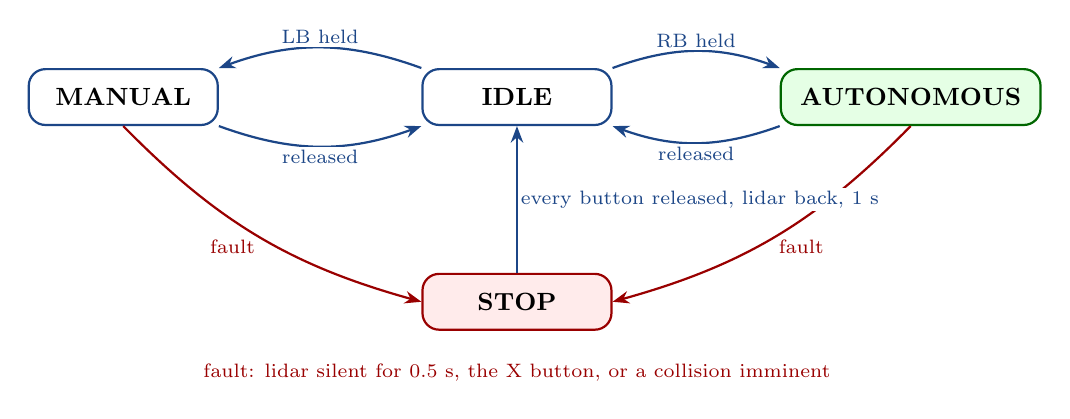
\begin{tikzpicture}[font=\small]
  \node[state] (idle) at (0,0) {IDLE};
  \node[state] (manual) at (-5,0) {MANUAL};
  \node[go] (auto) at (5,0) {AUTONOMOUS};
  \node[stop] (stop) at (0,-2.6) {STOP};
  \draw[flow] (idle.north west) to[bend right=20] node[lbl,above]{LB held} (manual.north east);
  \draw[flow] (manual.south east) to[bend right=20] node[lbl,below]{released} (idle.south west);
  \draw[flow] (idle.north east) to[bend left=20] node[lbl,above]{RB held} (auto.north west);
  \draw[flow] (auto.south west) to[bend left=20] node[lbl,below]{released} (idle.south east);
  \draw[flow,red!60!black] (manual.south) to[bend right=15] node[lbl,below left,text=red!60!black]{fault} (stop.west);
  \draw[flow,red!60!black] (auto.south) to[bend left=15] node[lbl,below right,text=red!60!black]{fault} (stop.east);
  \draw[flow] (stop.north) -- node[lbl,right]{every button released, lidar back, 1 s} (idle.south);
  \node[font=\scriptsize\color{red!60!black}] at (0,-3.5) {fault: lidar silent for 0.5 s, the X button, or a collision imminent};
\end{tikzpicture}
\end{center}

\begin{itemize}
  \item \textbf{IDLE}: the car sits. Your stack is running and publishing \texttt{/drive}; it goes nowhere.
  \item \textbf{MANUAL}, LB held: the sticks drive. For positioning the car and checking wiring.
  \item \textbf{AUTONOMOUS}, RB held: your \texttt{/drive} reaches the wheels, clipped to the mode's cap.
  \item \textbf{STOP}: brakes. Entered when the lidar goes silent, the stop button is pressed, or a
  collision is imminent; left for IDLE only once every button is released and the sensors are back.
  \item Release either button: zero speed, which is a brake, within a third of a second.
\end{itemize}

\textbf{In the simulator}, \cmd{./feb up -{}-deadman -{}-driver NAME} runs the same rules with the
keyboard as the pad: hold SPACE for RB, hold M for LB with the arrows driving, X for the stop
button, Q to quit. The keys go to the \emph{terminal} you ran it in, so keep that window focused,
not the simulator's. The nodes' output goes to \cmd{./feb logs -f} in another terminal. Run every
driver this way once before it goes near the car.

\textbf{Your stack and the state.} The button never starts or stops your stack; it only gates its
output. So anything that remembers, an MPC's warm start, a localiser, an integrator, is stale when
RB goes down. The rule: \emph{on AUTONOMOUS, start clean}. \texttt{feb\_mission}, a forty-line
package in the starter kit, turns \texttt{/feb/state} into two hooks, \texttt{on\_go} and
\texttt{on\_stop}, and a live flag; a stack with memory fills them in. The gap follower needs none
of it.

\section{Score and submit}

\begin{lstlisting}
./feb practice --driver my_driver        # every practice track of its kind, competition rules; --headless to hide the window
./feb submit --dry-run                   # what would be posted
./feb submit
\end{lstlisting}

\texttt{practice} runs each track in its own clean container the way the competition does: a
warm-up lap and ten timed laps, 300~s limit, 10~s per collision and disqualified above ten, at the
10~Hz scoring rate. The simulator window shows unless you add \cmd{-{}-headless}. Each run lands in
\file{runs/<id>/} with a result file, a bag and the logs.

Both commands check that your copy of \file{feb-racing} is current: \texttt{practice} prints a
line when it is behind, \texttt{submit} refuses until you run \cmd{./feb update} (the board reruns
every result on the current harness, so a stale one may not verify); \cmd{-{}-allow-stale}
overrides. Offline, nothing is checked.

\texttt{submit} does two things from one command. It posts every clean run (finished, no
collisions) not yet posted to the scoreboard as one pull request to \file{feb-racing}, which
checks and merges itself; the site rebuilds and your time appears, unverified until the nightly
rerun. And it copies your driver's packages, the \texttt{packages:} list in its card, into the
team repo \file{feb-stack} under \file{drivers/<your name>/}, on a branch named after you, with a
pull request to main that the lead reviews. Nothing changed since last time: nothing is pushed.
\cmd{-{}-no-code} and \cmd{-{}-no-results} pick one half.

\begin{center}
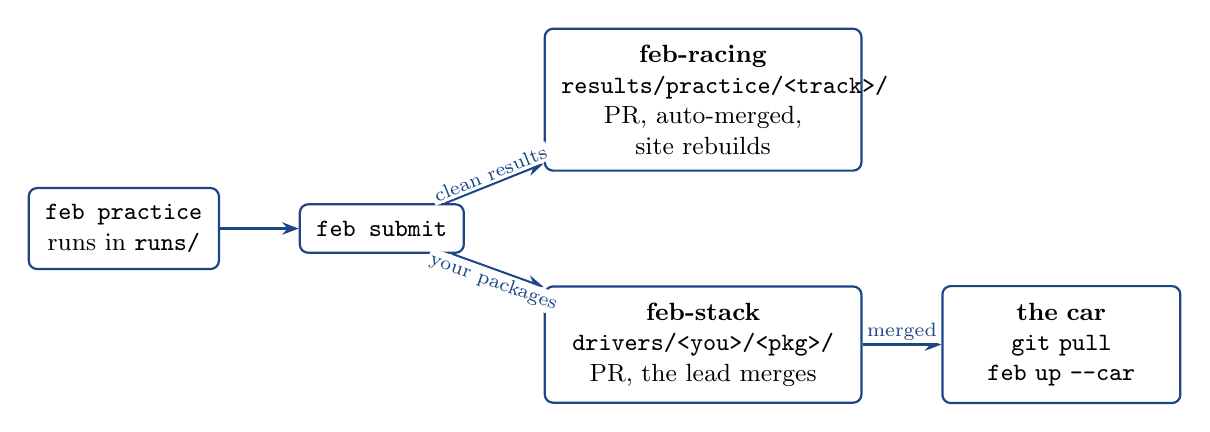
\begin{tikzpicture}[node distance=6mm and 10mm, font=\small]
  \node[box] (prac) {\cmd{feb practice}\\runs in \file{runs/}};
  \node[box, right=of prac] (sub) {\cmd{feb submit}};
  \node[box, above right=4mm and 10mm of sub, text width=36mm] (res) {\textbf{feb-racing}\\\file{results/practice/<track>/}\\PR, auto-merged, site rebuilds};
  \node[box, below right=4mm and 10mm of sub, text width=36mm] (code) {\textbf{feb-stack}\\\file{drivers/<you>/<pkg>/}\\PR, the lead merges};
  \node[box, right=of code, text width=26mm] (car) {\textbf{the car}\\\cmd{git pull}\\\cmd{feb up -{}-car}};
  \draw[flow] (prac) -- (sub);
  \draw[flow] (sub) -- node[lbl,above,sloped]{clean results} (res);
  \draw[flow] (sub) -- node[lbl,below,sloped]{your packages} (code);
  \draw[flow] (code) -- node[lbl,above]{merged} (car);
\end{tikzpicture}
\end{center}

\textbf{The team repo.} \file{FEBAutonomous/feb-stack} holds the drivers that drive, one folder
per person under \file{drivers/}, and one copy of the shared packages under \file{shared/}
(\texttt{feb\_mission}, \texttt{feb\_cone\_ordering}). Nobody edits it by hand. To run a
teammate's merged driver in your simulator: \cmd{./feb up -{}-ws \textasciitilde/FEB/feb-stack
-{}-driver theirs}.

\part{The car}

\section{From a merged driver to the wheels}

The Jetson on the car has the same box, the same \file{\textasciitilde/FEB} folder, and the pad's
dongle. Nothing on a laptop or on GitHub is needed to drive; the laptop is only a terminal.

\textbf{Start-up.} Gamepad on \emph{first}, then battery in, SW1 on, a minute for the Jetson to boot.
Then a terminal on it, whichever fits:

\begin{tabularx}{\linewidth}{lX}
\toprule
Where & How \\
\midrule
no internet (track, corridor) & 45 s after boot the car is Wi-Fi network \texttt{feb-car}, password \texttt{febautonomous}; join it, then \cmd{ssh feb@10.42.0.1} \\
a known Wi-Fi around & the car joins it; \cmd{ssh feb@feb-car} from any laptop on the team tailnet, or its address on that network \\
a USB-C cable to the Jetson & \cmd{ssh feb@192.168.55.1} \\
\bottomrule
\end{tabularx}

\medskip
Password \texttt{feb}. Then:

\begin{lstlisting}
cd ~/FEB/feb-stack && git pull
cd ~/FEB/feb-racing
./feb up --car --driver my_driver --mode-name inspection
\end{lstlisting}

Wait for \emph{Connected to VESC} and \emph{Opened joystick} in the output. If the pad came on
after that, Ctrl-C and run it again: the joystick node only looks once. Ctrl-C ends the run, and
so does losing the ssh connection, which is the safe way round; for a long demo put \cmd{nohup}
in front and \cmd{\&} at the end, the bumper still stops the car.

On the car the workspace is \file{feb-stack} by default, so every merged driver is built and the
named one launches. A driver that is nowhere in the workspace is looked for in the starter kit next,
so \cmd{./feb up -{}-car -{}-driver feb\_driver -{}-mode-name inspection} works on a car with no
merged drivers yet; \cmd{-{}-ws FOLDER} points at any other workspace. Either way the launch is the same: the VESC, lidar and gamepad drivers instead of the simulator, the supervisor
with the dead-man required and the mode's cap, then your launch file with your car yaml on top.
LB held, a human drives; RB held, your code drives; let go, it stops. Foxglove on a laptop at
\texttt{ws://<the car>:8765} shows the same panels as in the simulator. First drive in
\texttt{inspection}, then \texttt{trackdrive}. The lead's own notes on the car, wiring to first
drive, are \file{docs/build-car.md}.

\section{When something is wrong}

Setting up:

\begin{tabularx}{\linewidth}{lX}
\toprule
Symptom & Fix \\
\midrule
\texttt{Cannot connect to the Docker daemon} & Docker Desktop is not running; open it, wait for the whale icon to settle \\
the car stops with \texttt{STOP: no lidar} every half minute (Windows) & the box's clock is jumping: a second WSL Ubuntu, or Windows itself, keeps resetting it. Windows Settings, Time, \emph{Set time automatically} on; in every other WSL Ubuntu \cmd{sudo systemctl disable -{}-now systemd-timesyncd}; then \cmd{wsl -{}-shutdown} and start Docker Desktop again \\
Docker Desktop will not start (Windows) & \cmd{wsl -{}-update} in PowerShell, reboot, open Docker Desktop again: an old WSL stops its engine \\
\texttt{this clone sits directly in /home/...} & the clone needs a folder of its own: \cmd{mkdir \textasciitilde/FEB \&\& mv \textasciitilde/feb-racing \textasciitilde/FEB/} \\
\texttt{unauthorized} while pulling the image & a stale \cmd{ghcr.io} login: \cmd{docker logout ghcr.io}, run setup again \\
\texttt{refusing to merge unrelated histories} & you pulled in the old clone; delete it and clone again (Setup) \\
\bottomrule
\end{tabularx}

\medskip
Running:

\begin{tabularx}{\linewidth}{lX}
\toprule
Symptom & Fix \\
\midrule
\texttt{already running} on \cmd{./feb up} & a previous run is still going, its terminal was closed: \cmd{./feb stop} \\
\texttt{no card.yaml with name '...'} & no card with that \cmd{name:} in \file{stack/} or the starter kit: \cmd{./feb new NAME}, section~\ref{sec:package} \\
\texttt{ros2: command not found} & you are in a laptop terminal: \cmd{./feb shell} \\
my node is not there & it did not build: \cmd{./feb logs -n 100}, or \cmd{colcon build} in the workspace and read it \\
the simulator says not connected & the house nodes are still starting; \cmd{./feb logs -f} \\
\texttt{port is already allocated} & another box holds the port: \cmd{./feb reset} \\
\texttt{mounts denied} (Mac) & \file{\textasciitilde/FEB} is outside \file{/Users}: move it \\
the browser desktop will not connect & reload; still nothing, \cmd{./feb reset} \\
nothing is clean enough to submit & a run with a collision is not posted by default; drive slower, or \cmd{-{}-all} \\
anything weird & \cmd{./feb reset}: thirty seconds, nothing of yours is in there \\
\bottomrule
\end{tabularx}

\appendix
\section{Every track}\label{sec:tracks}

\cmd{./feb up -{}-track FOLDER} and \cmd{./feb practice -{}-track FOLDER} take the folder name; every track is in
\file{tracks/}, one folder each, with its picture. Qualifying tracks are the ones \cmd{feb practice} runs by
default and the board scores: \texttt{loop} and \texttt{porto} for walls drivers, \texttt{loop\_cones} for cones
drivers. The rest are practice: \cmd{-{}-track all} runs every track of the driver's kind.

\begin{tabularx}{\linewidth}{llXl}
\toprule
Folder & Kind & Name & Direction \\
\midrule
\multicolumn{4}{l}{\textit{FEB, ours, walls}} \\
\texttt{circuit} & walls & FEB Circuit & ccw \\
\texttt{esses} & walls & FEB Esses & ccw \\
\texttt{loop \textbf{(qualifying)}} & walls & FEB Loop & ccw \\
\midrule
\multicolumn{4}{l}{\textit{FEB, cone edition}} \\
\texttt{circuit\_cones} & cones & FEB Circuit (cones) & cw \\
\texttt{esses\_cones} & cones & FEB Esses (cones) & cw \\
\texttt{loop\_cones \textbf{(qualifying)}} & cones & FEB Loop (cones) & cw \\
\midrule
\multicolumn{4}{l}{\textit{RoboRacer league, walls}} \\
\texttt{porto \textbf{(qualifying)}} & walls & Porto (legacy RoboRacer) & ccw \\
\texttt{rr\_berlin} & walls & Berlin & ccw \\
\texttt{rr\_vegas} & walls & Vegas & ccw \\
\midrule
\multicolumn{4}{l}{\textit{F1 circuits, walls}} \\
\texttt{interlagos} & walls & Interlagos (1:10) & ccw \\
\texttt{monza} & walls & Monza (1:10) & ccw \\
\texttt{silverstone} & walls & Silverstone (1:10) & ccw \\
\texttt{spa} & walls & Spa-Francorchamps (1:10) & ccw \\
\texttt{spielberg} & walls & Spielberg (1:10) & ccw \\
\midrule
\multicolumn{4}{l}{\textit{F1 circuits, cones}} \\
\texttt{interlagos\_cones} & cones & Interlagos (1:10, cones) & cw \\
\texttt{monza\_cones} & cones & Monza (1:10, cones) & cw \\
\texttt{silverstone\_cones} & cones & Silverstone (1:10, cones) & cw \\
\texttt{spa\_cones} & cones & Spa-Francorchamps (1:10, cones) & cw \\
\texttt{spielberg\_cones} & cones & Spielberg (1:10, cones) & cw \\
\midrule
\multicolumn{4}{l}{\textit{Formula Student layouts, cones}} \\
\texttt{fs\_boa\_constrictor} & cones & FS boa constrictor (EUFS) & ccw \\
\texttt{fs\_bone} & cones & FS bone (EUFS) & ccw \\
\texttt{fs\_comp\_2021} & cones & FS comp 2021 (EUFS) & cw \\
\texttt{fs\_hairpins\_increasing\_difficulty} & cones & FS hairpins (EUFS) & cw \\
\texttt{fs\_peanut} & cones & FS peanut (EUFS) & ccw \\
\texttt{fs\_rectangle} & cones & FS rectangle (EUFS) & ccw \\
\texttt{fs\_small\_track} & cones & FS small track (EUFS) & cw \\
\texttt{fsg} & cones & FS Germany & cw \\
\texttt{fsi} & cones & FS Italy & cw \\
\bottomrule
\end{tabularx}

\end{document}
